\documentclass[tikz]{standalone}
\usepackage{tikz}  
\usepackage{../preamble_lat}

\usetikzlibrary{arrows,arrows.meta}
\usepackage{xcolor}

\definecolor{c1}{RGB}{51,153,255}
\definecolor{c2}{RGB}{255,178,102}

\begin{document}

\begin{tikzpicture}
\newcommand{\CyclicFolder}{../Numerics/Sampling_Cyclic}
\newcommand{\NoinvFolder}{../Numerics/Sampling_noinv_p}
\newcommand{\HinvFolder}{../Numerics/Sampling_hinv_p}


\node at (0,0) {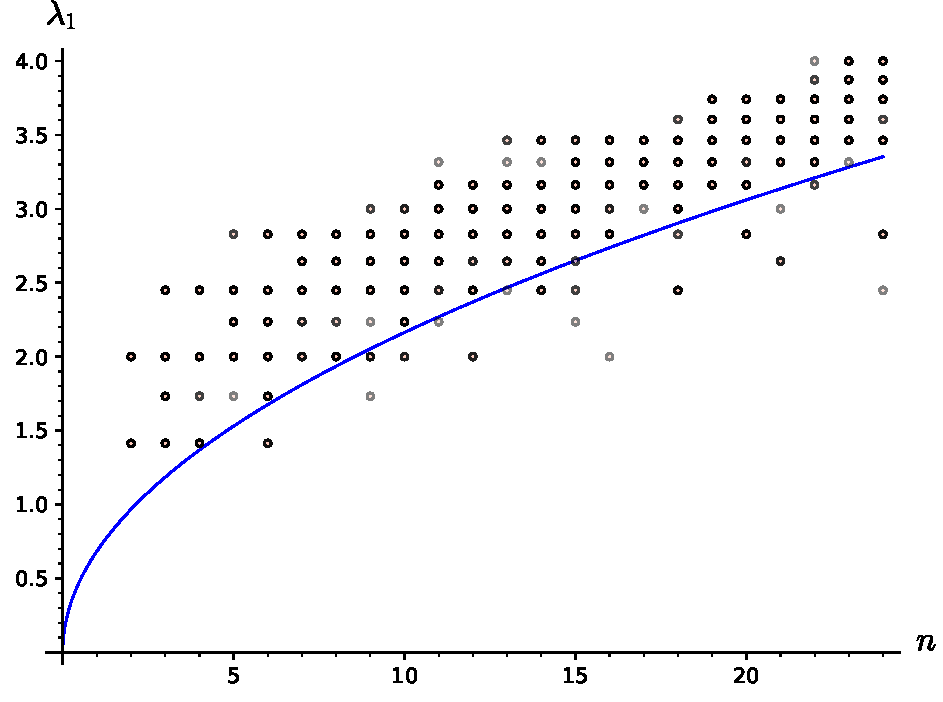
\includegraphics{\CyclicFolder/Cyclic_samples_HKZlambda_q4.pdf}};
\node at (16,0) {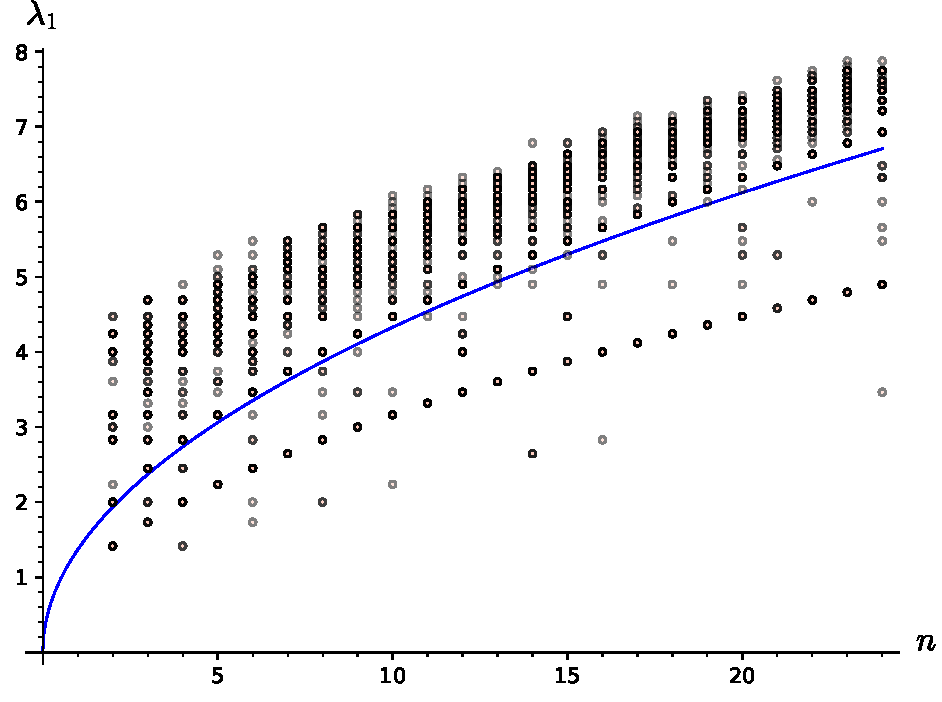
\includegraphics{\CyclicFolder/Cyclic_samples_HKZlambda_q16.pdf}};
\node at (32,0) {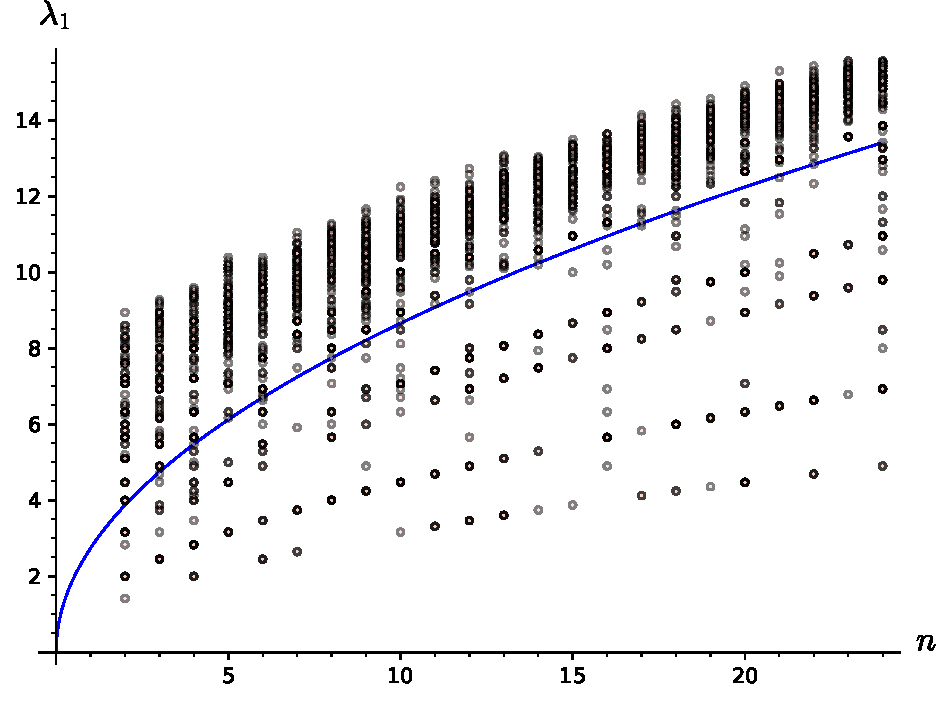
\includegraphics{\CyclicFolder/Cyclic_samples_HKZlambda_q64.pdf}};
\node at (48,0) {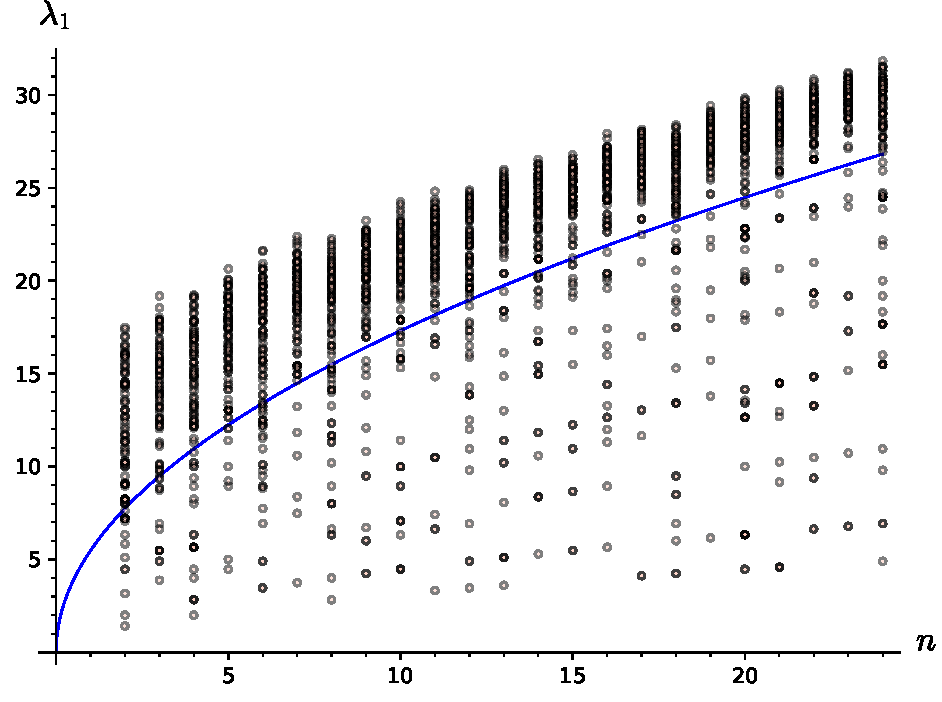
\includegraphics{\CyclicFolder/Cyclic_samples_HKZlambda_q256.pdf}};
\node at (64,0) {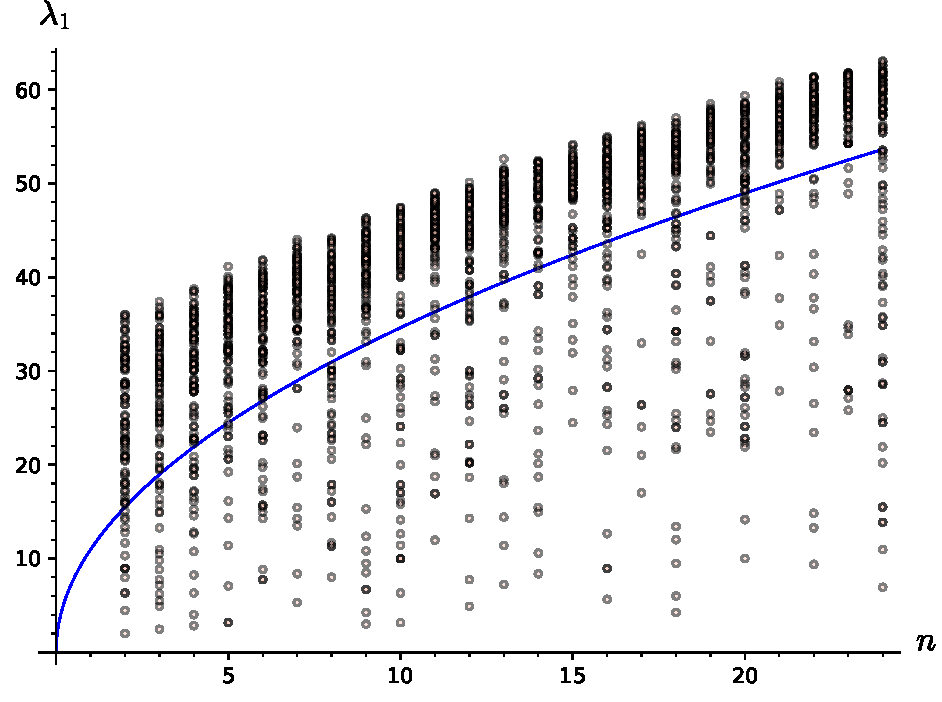
\includegraphics{\CyclicFolder/Cyclic_samples_HKZlambda_q1024.pdf}};


\node at (0,-12) {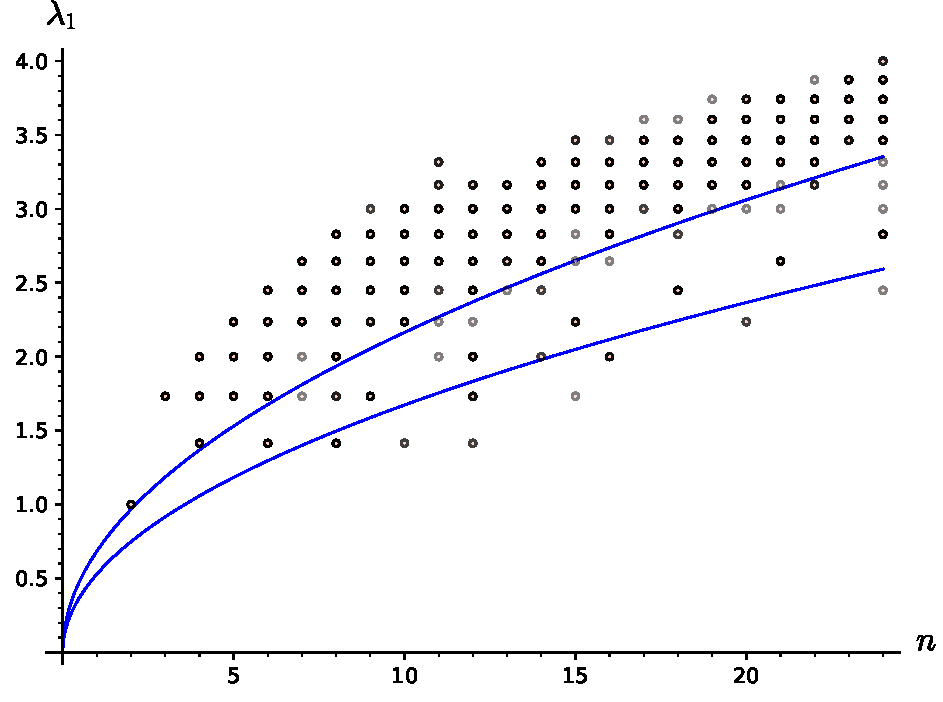
\includegraphics{\NoinvFolder/NTRU_samples_noinv_pub_HKZlambda_q4.pdf}};
\node at (16,-12) {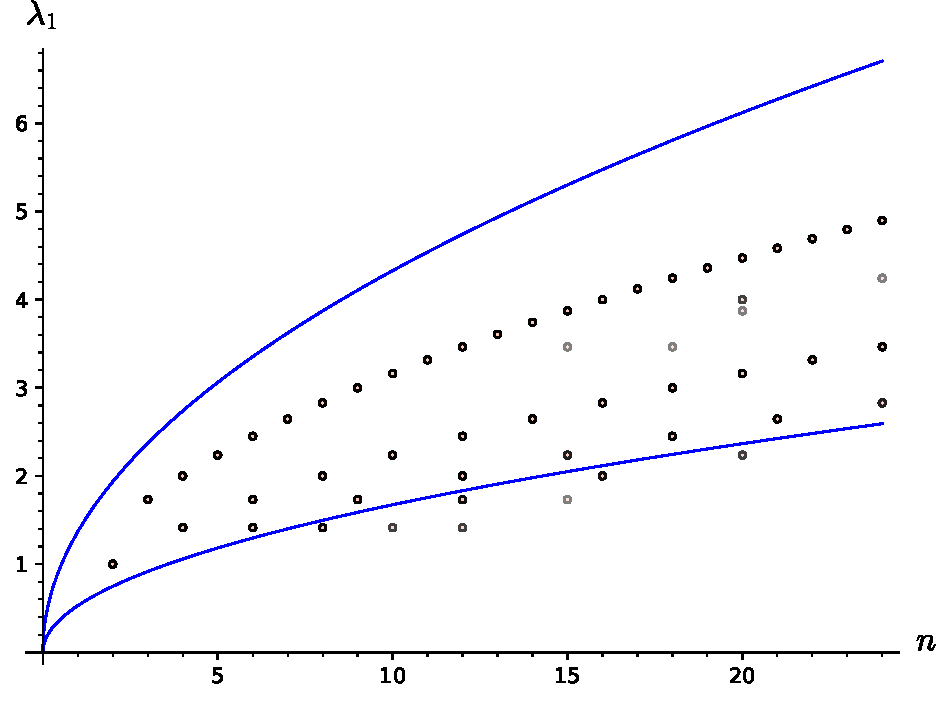
\includegraphics{\NoinvFolder/NTRU_samples_noinv_pub_HKZlambda_q16.pdf}};
\node at (32,-12) {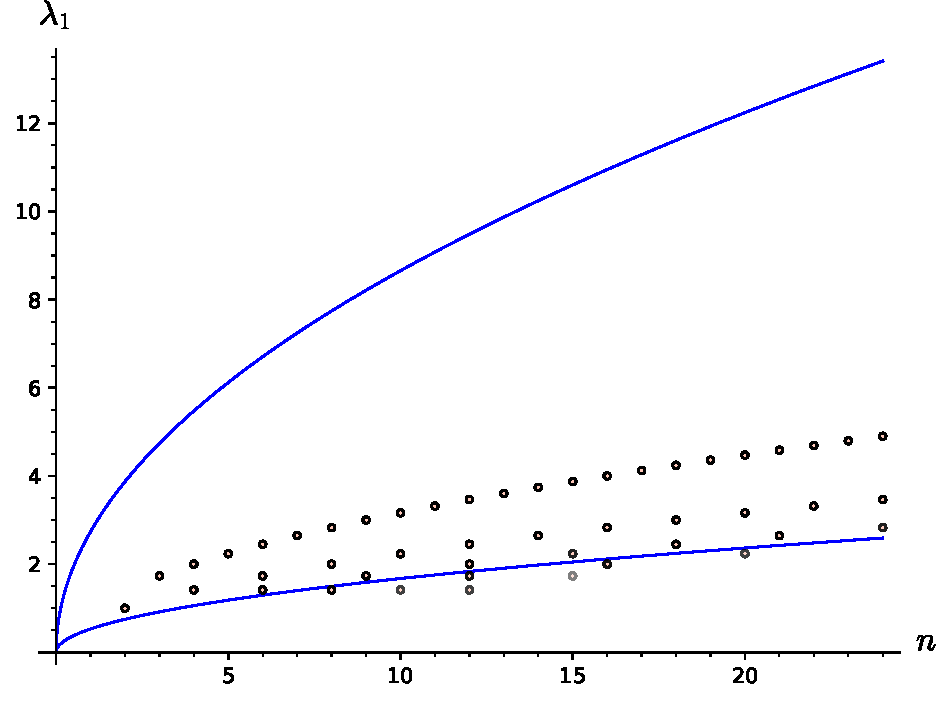
\includegraphics{\NoinvFolder/NTRU_samples_noinv_pub_HKZlambda_q64.pdf}};
\node at (48,-12) {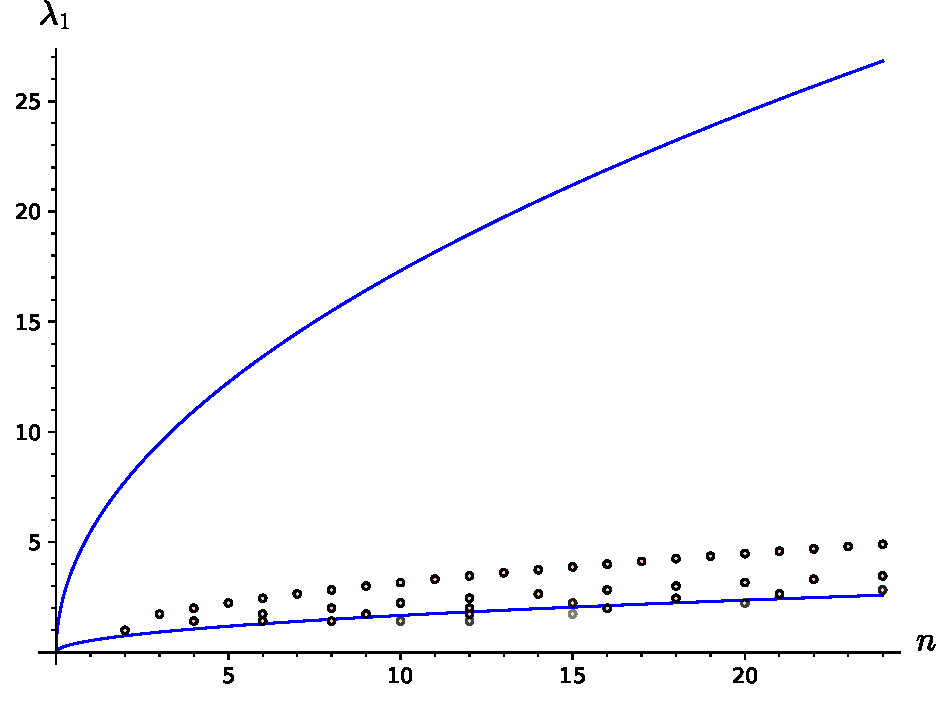
\includegraphics{\NoinvFolder/NTRU_samples_noinv_pub_HKZlambda_q256.pdf}};
\node at (64,-12) {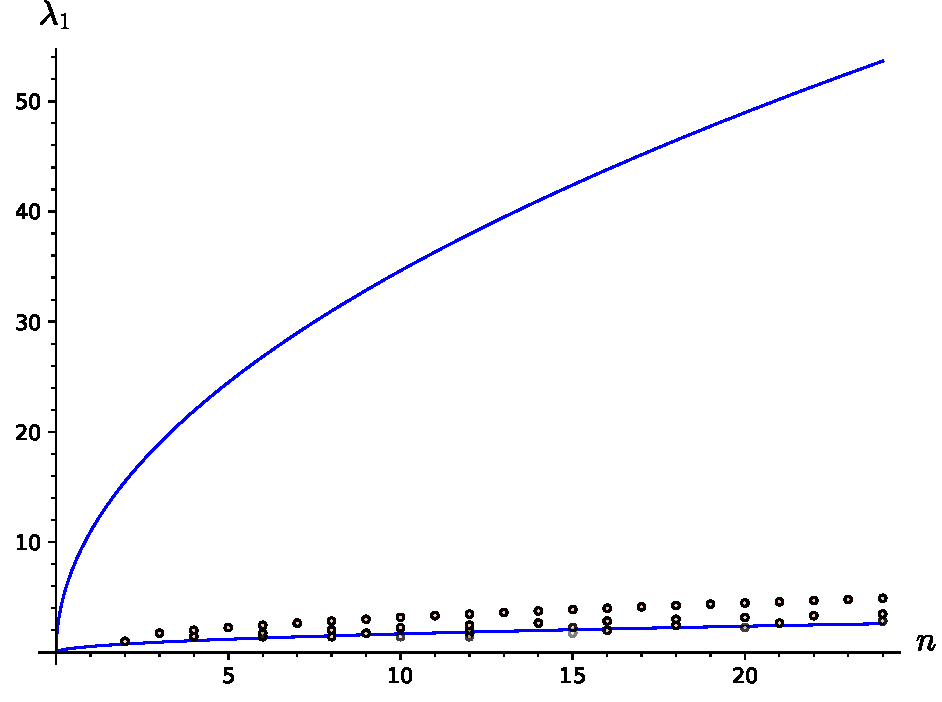
\includegraphics{\NoinvFolder/NTRU_samples_noinv_pub_HKZlambda_q1024.pdf}};



\node at (0,-24) {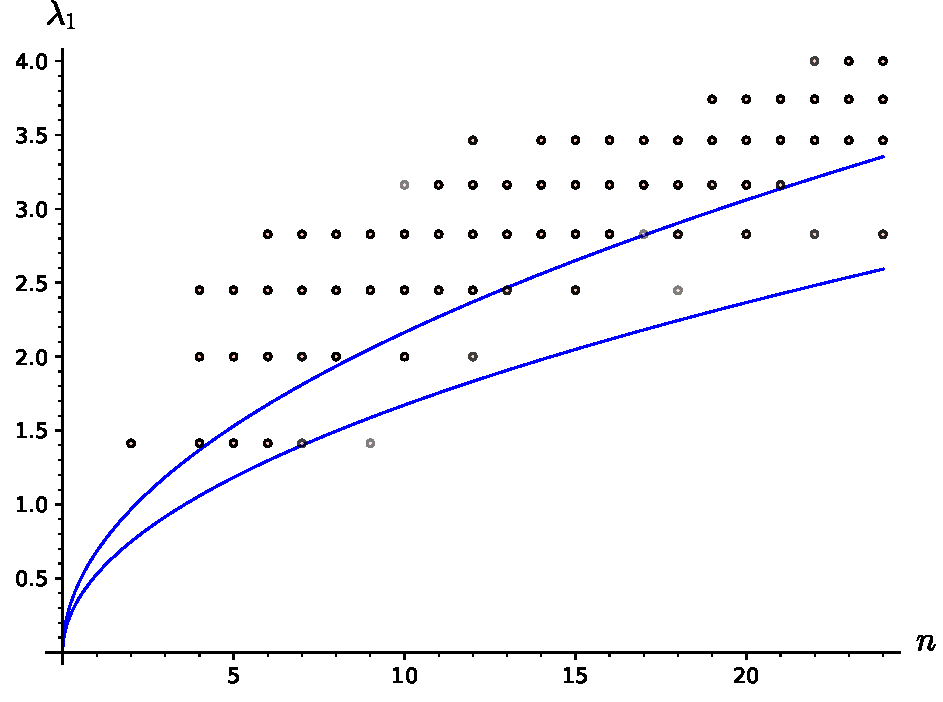
\includegraphics{\HinvFolder/NTRU_samples_hinv_pub_HKZlambda_q4.pdf}};
\node at (16,-24) {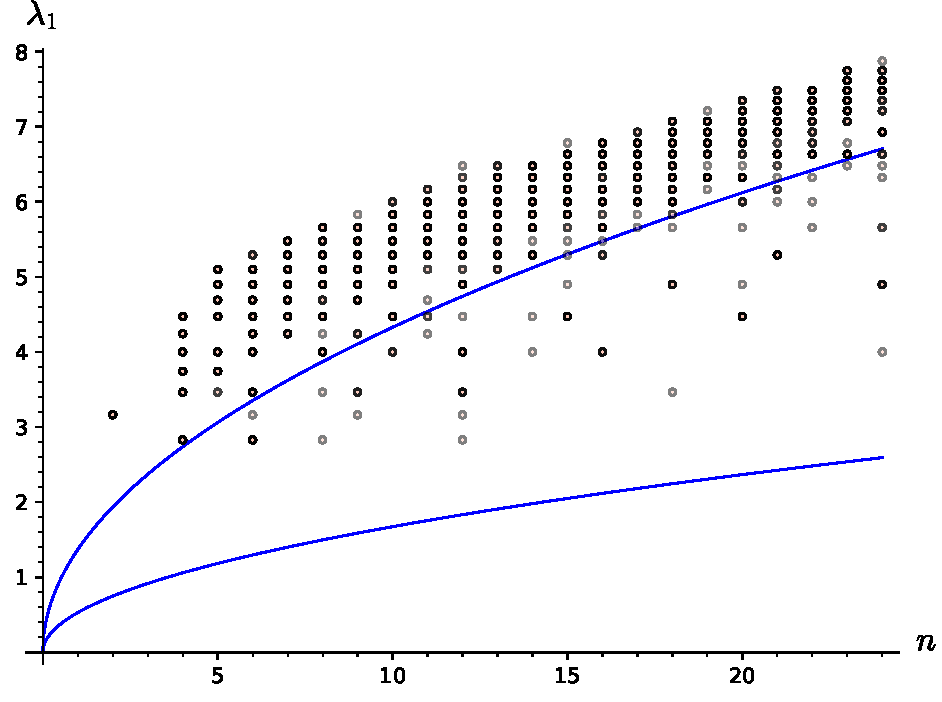
\includegraphics{\HinvFolder/NTRU_samples_hinv_pub_HKZlambda_q16.pdf}};
\node at (32,-24) {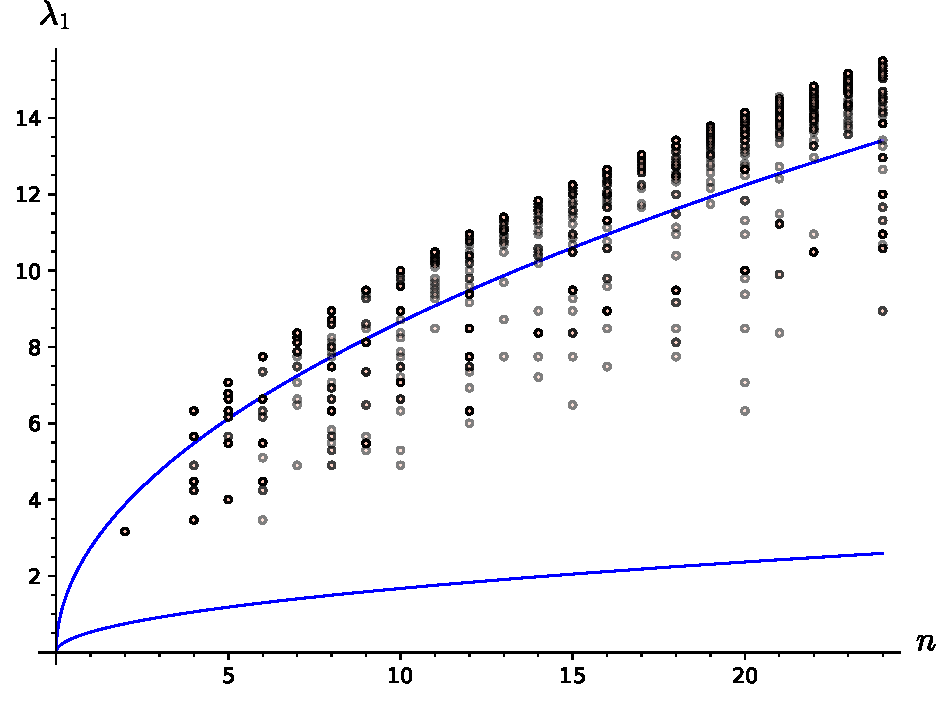
\includegraphics{\HinvFolder/NTRU_samples_hinv_pub_HKZlambda_q64.pdf}};
\node at (48,-24) {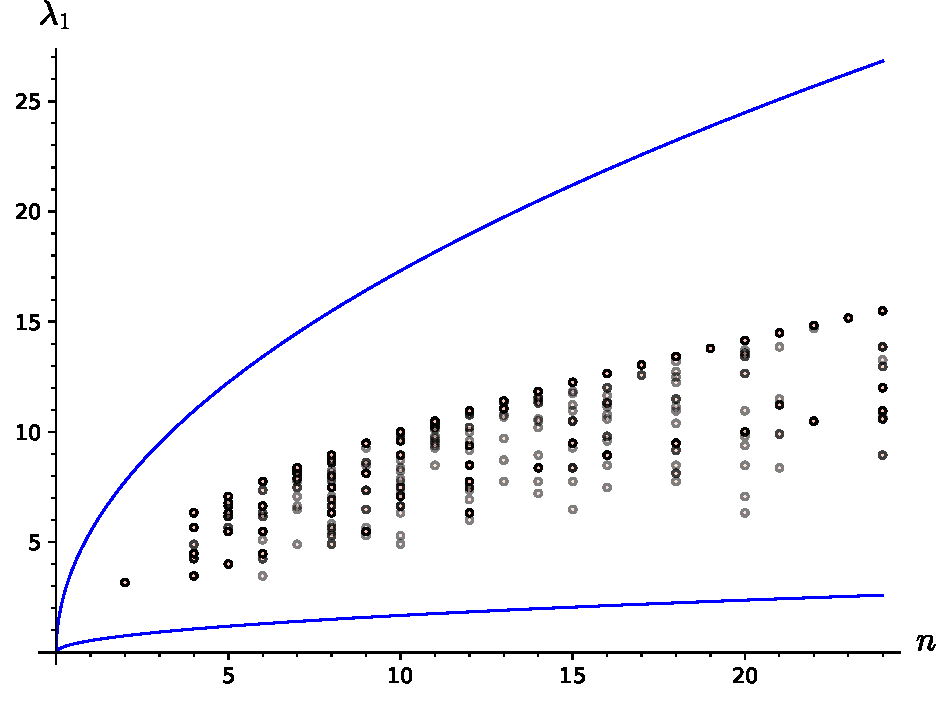
\includegraphics{\HinvFolder/NTRU_samples_hinv_pub_HKZlambda_q256.pdf}};
\node at (64,-24) {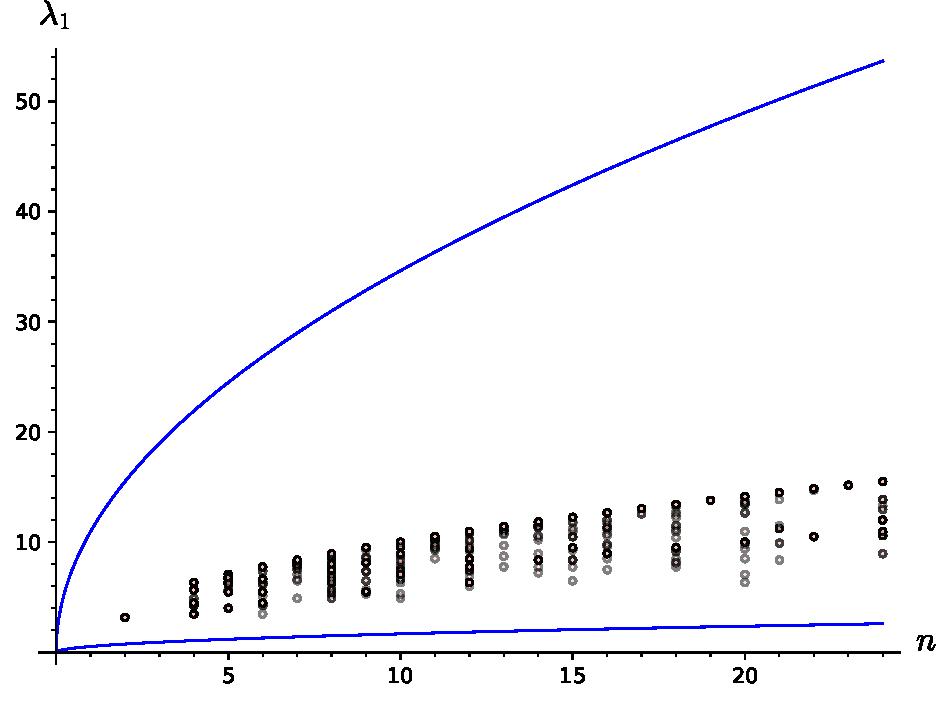
\includegraphics{\HinvFolder/NTRU_samples_hinv_pub_HKZlambda_q1024.pdf}};
\node[scale=4] at (-20,  6) {$ a)$};
\node[scale=3] at (-15,  0) {$\begin{aligned} h  \sim \mathbb{Z}_q[x] / \langle x^n-1\rangle \end{aligned}$};
\node[scale=4] at (-20,  -6) {$ b)$};
\node[scale=3] at (-14,  -12){$\begin{aligned}f &\sim 1+D(d,d) \\&\hspace{.5cm} \text{invertible} \,  \mod q \\ g &\sim D(d,d)  \\ d&=\lfloor n/3 \rfloor \end{aligned}$}; 
% \node[scale=3] at (-14,  -13){$g \sim T(d,d)$};
\node[scale=4] at (-20,  -18) {$ c)$};
\node[scale=3] at (-14,  -24){$\begin{aligned}f &\sim 1+D(d,d) \\&\hspace{.5cm} \text{invertible}\,  \mod q \\ g &\sim D(d+1,d)  \\ h &=g/f \\&\hspace{.5cm}\text{invertible}\,  \mod q  \\ d&=\lfloor n/3 \rfloor\end{aligned} $}; 

\node[scale=3] at (0,7) {$q=4$};
\node[scale=3] at (16,7) {$q=16$};
\node[scale=3] at (32,7) {$q=64$};
\node[scale=3] at (48,7) {$q=256$};
\node[scale=3] at (64,7) {$q=1024$};
\end{tikzpicture}

\end{document}